\subsection{\label{sub:\projectname-AmesB} \textsf{AmesB}}

\paragraph{Símbol}

\begin{center} \bsfsymbol{AmesB} \end{center}

\paragraph{Entrades i sortides}

\begin{where}
\item[\nodenamebit{sigA}] Signe del primer factor
\item[\nodenamerange{A}{3}{0}] Mòdul del primer factor (BCD)
\item[\nodenamebit{sigB}] Signe del segon factor
\item[\nodenamerange{B}{3}{0}] Mòdul del segon factor (BCD)
\item[\nodenamebit{sigAmesB}] Signe del producte
\item[\nodenamerange{AmesB}{7}{0}] Mòdul del producte (BCD)
\end{where}

\paragraph{Funció}

Sumador BCD d'una xifra amb signe, amb resultat en dues xifres.

Retorna a les sortides $sigAmesB$ i $AmesB$ el signe i mòdul de la suma de $sigA$, $A$ amb $sigB$, $B$.

\paragraph{Inespecificacions}


La sortida no està definida si $A$ o $B$ no pertanyen al seu codi.


\paragraph{Implementació}

\vhdlisting{AmesB}



Primer, s'expressa $A$ i $B$ en Ca2 de 5~bits, i es desen en senyals intermedis \mintinline{vhdl}|signed|.

Llavors, s'estenen els senyals intermedis a 8~bits, es sumen
i es passen a vector lògic per a obtenir el resultat de la suma en Ca2.

Finalment, s'utilitza \textsf{CA2\_BCD\_8B} per a extreure el mòdul del resultat en BCD de dues xifres,
i es retorna juntament amb el signe a les sortides corresponents.

\paragraph{Simulació}

\begin{contendfig}
  \begin{center}
    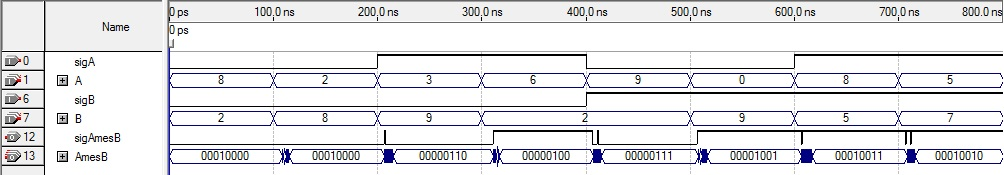
\includegraphics[scale=0.55]{../\projectname/assets/vwf/AmesB.jpg}
  \end{center}
  \caption{\label{fig:sim-\projectname-AmesB} Simulació per al bloc \textsf{AmesB}}
\end{contendfig}

La simulació del bloc es pot veure a la figura~\ref{fig:sim-\projectname-AmesB} (pàgina~\pageref{fig:sim-\projectname-AmesB}).

% FIXME

\vspace{1cm}
